\documentclass[aspectratio=169,
				xcolor=table]{beamer}

% Load general definitions
\usepackage[utf8]{inputenc}
%\usepackage[T1]{fontenc}
\usepackage[brazil]{babel}
\usepackage{amsmath}
\usepackage{amsfonts}
\usepackage{amssymb}
\usepackage{graphicx}
\usepackage{verbatim}
\usepackage{cancel}
\usepackage{askmaps}
\usepackage{tabularx}
\usepackage[table]{xcolor}
%\usepackage{tikz}
\usepackage{multirow}
\usepackage{mathtools}
\usepackage{color, colortbl}
\usepackage{etoolbox}
\usepackage{pbox}
\usepackage{changepage}
\usepackage{xpatch}
\usepackage{array}
\usepackage{marvosym}
\usepackage{tabu}
\usepackage{multicol}
\usepackage{listings}
\usepackage{underscore}
\usepackage{filecontents}
\usepackage[]{algorithm2e}
\usepackage{ragged2e}

\newcolumntype{P}[1]{>{\centering\arraybackslash}m{#1}}
\definecolor{Gray}{gray}{0.75}
\definecolor{Gray2}{gray}{0.85}

\definecolor{lightBlue}{HTML}{DAE8FC}
\definecolor{Blue}{RGB}{51, 51, 204}

%\useinnertheme[lily]{rounded}
\usetheme{UniEvangelica}
%\usetheme{Copenhagen}
%\usetheme{Berlin}
%\usecolortheme{dolphin}
\tolerance=1
\emergencystretch=\maxdimen
\hyphenpenalty=10000
\hbadness=10000

\setbeamertemplate{navigation symbols}{}%remove navigation symbols


\let\olditem=\item% 
\renewcommand{\item}{\olditem \justifying}%
\def\center{\trivlist \centering\item\relax}
\def\endcenter{\endtrivlist}

\setbeamertemplate{itemize/enumerate body begin}{\large}
\setbeamertemplate{itemize/enumerate subbody begin}{\large}

\setbeamertemplate{itemize item}{\raisebox{0.1ex}{$\blacktriangleright$}\hskip0.1em}
\setbeamertemplate{itemize subitem}{\raisebox{0.1ex}{$\blacktriangleright$}\hskip0.1em}

\newcommand{\greenarrow}{\textcolor{green}{\rotatebox[origin=c]{180}{\MVArrowDown}}}

\newcommand{\redarrow}{\textcolor{red}{\MVArrowDown}}

%\newcommand{\ftable}{
%	\begin{table}
%		\large
%		\centering
%		\rowcolors{1}{\ifnumless{\rownum}{2}{Blue}{lightBlue}}{}
%}

\newenvironment{eftable}{
	\begin{table}
		\large
		\centering
		\rowcolors{1}{}{Blue}
		\rowcolors{1}{\ifnumless{\rownum}{2}{Blue}{lightBlue}}{}
	}
	{
	\end{table}
}


%\setbeamertemplate{frametitle}
%{
%	%\vspace*{-2em}	
%	\insertframetitle
%
%	 %\textcolor{white}{\LARGE \insertframetitle}
%
%}
% Specific definitions
\institute[]{\uppercase{Engenharia de Software}}
\title[]{Arquitetura e Organização de Computadores}
\subtitle[]{\uppercase{Estrutura do Computador}}
\author[]{Prof. Alexandre Tannus}
\date{}
\AtBeginSection{\frame{\tableofcontents[currentsection]}}

\begin{document}

	\begin{frame}
		\titlepage
	\end{frame}

	\begin{frame}{Objetivos}
		\begin{itemize}
			\item Conhecer a estrutura do computador
			\vspace{1em}
			\item Definir a função de cada parte integrante do computador
			\vspace{1em}
			\item Compreender os modelos de arquitetura e suas particularidades
		\end{itemize}
	\end{frame}
	
%	\begin{frame}{Metodologia}
%		\begin{itemize}
%			\item O tema da aula é exposto pelo professor em sala de aula. Os alunos interagem durante a apresentação para resolução de dúvidas e exposição de questionamentos relevantes ao tema, os quais podem ser sanados diretamente pelo professor ou serem colocados em discussão pela turma. 
%			\vspace{1em}
%			\item Ao final da exposição do conteúdo são resolvidos exercícios de fixação, para melhor compreensão do tema. As questões podem ser retiradas de concursos públicos, ENADE, POSCOMP ou de autoria do próprio professor.
%		\end{itemize}
%	\end{frame}

	\begin{frame}
		\tableofcontents		
	\end{frame}	
	
	\section{Introdução}
		
		\begin{frame}{Questionamentos}
			\begin{itemize}
				\item Quais partes compõem um sistema computacional?
				\vspace{1em}
				\item Qual a função básica de cada uma destas partes?
				\vspace{1em}
				\item Como elas se interconectam?
			\end{itemize}
		\end{frame}
		
		\begin{frame}{Introdução}
			\begin{itemize}
				\item Os computadores são formados por quatro estruturas básicas
				\begin{itemize}
					\item Unidade Central de Processamento (CPU - \textit{Central Processing Unit})
					\item Memórias
					\item Dispositivos de entrada e saída (E/S ou I/O - \textit{Input/Output})
					\item Barramentos
				\end{itemize}
			\end{itemize}
		\end{frame}
		
		\begin{frame}{Estrutura do Computador}
			\begin{figure}
			\centering
				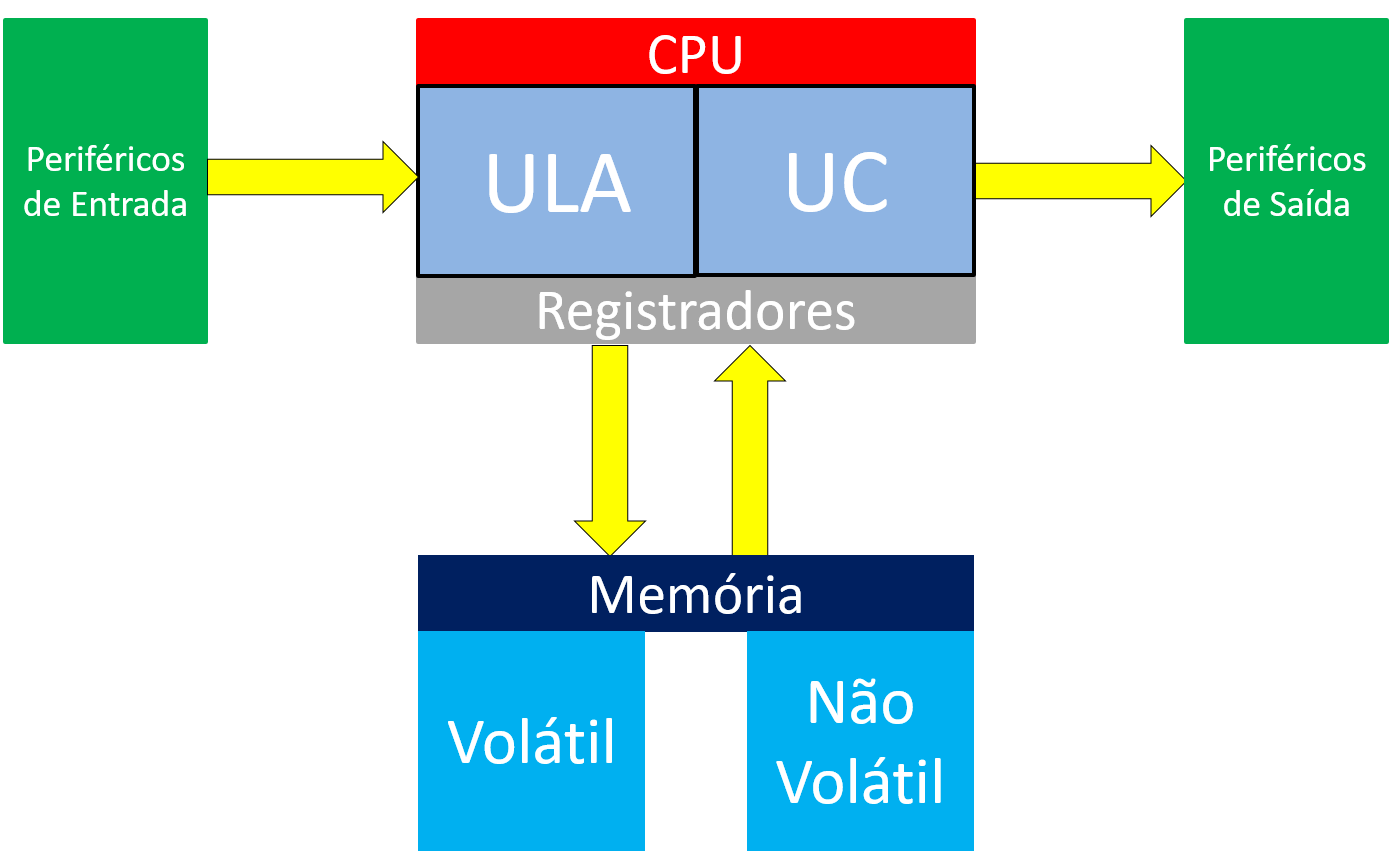
\includegraphics[width=0.7\textwidth, keepaspectratio]{../figs/cap04/estrutura.png} 
			\end{figure}
		\end{frame}
			
	\section{Unidade Central de Processamento}
	
		\begin{frame}
			\frametitle{Unidade Central de Processamento}
			\begin{itemize}
				\item Responsável pelo processamento de dados do sistema

				\item Composta por
				\begin{itemize}
					\item Unidade Lógica Aritmética (ULA)
					\item  Unidade de Controle (UC)
					\item  Registradores
				\end{itemize}
			\end{itemize}
		\end{frame}
		
		\begin{frame}{CPU - Unidade Lógica Aritmética}
			\begin{columns}
				\begin{column}{0.6\textwidth}
					\begin{itemize}
						\item Realiza as operações lógicas e aritméticas
						\begin{itemize}
							\item NOT, OR, AND
							\item Adição, Subtração
							\item Comparação
							\item Deslocamento
						\end{itemize}				
					\end{itemize}				
				\end{column}
				\begin{column}{0.4\textwidth}
				
					\begin{figure}
					\centering
						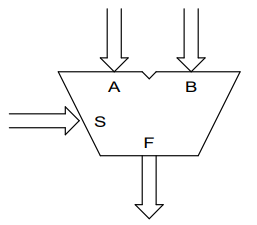
\includegraphics[width=0.9\textwidth, keepaspectratio]{../figs/cap04/ula} 
					\end{figure}
				\end{column}
			\end{columns}

			\begin{flushright}
				\begin{minipage}{0.7\textwidth}
					\vspace{-4em}
				\end{minipage}
			\end{flushright}

		\end{frame}
		
		\begin{frame}{CPU - Unidade de Controle}
			\begin{itemize}
				\item Controla toda a operação do microprocessador
				\vspace{1em}
				\item Constituída por
				\begin{itemize}
					\item Circuito de temporização
					\item Controle e decodificação
					\item Decodificador de instruções
				\end{itemize}
			\end{itemize}
		\end{frame}
		
		\begin{frame}
			\frametitle{CPU - Registradores}
			\begin{itemize}
				\item Armazenam dados e instruções
				\vspace{1em}
				\item Baixa capacidade de armazenamento
				\vspace{1em}
				\item Alta velocidade de acesso
				\vspace{1em}
				\item Podem ser
				\begin{itemize}
					\item Propósito geral - operações lógicas e aritméticas
					\item Especiais - Acumuladores, \textit{Program Counter}, registrador de \textit{flags}, etc.
				\end{itemize}
				
			\end{itemize}
		\end{frame}
		
	\section{Memórias}
	
		\begin{frame}
			\frametitle{Memórias}
			\begin{itemize}
				\item Dispositivos para armazenamento de informações
				\vspace{1em}
				\item O armazenamento pode ser temporário ou permanente
				\vspace{1em}
				\item Tipos de memória 
				\begin{itemize}
					\item Volátil: RAM 
					\item Não volátil: ROM, Flash, EEPROM
				\end{itemize}

			\end{itemize}
		\end{frame}

		\begin{frame}
			\frametitle{Hierarquia de Memória}
			\begin{figure}
			\centering
				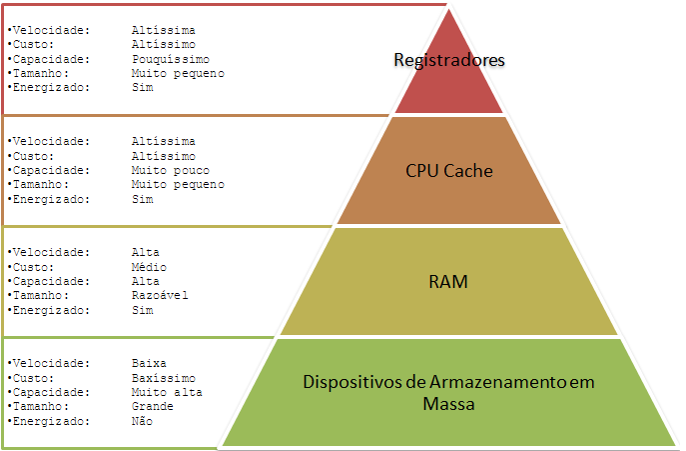
\includegraphics[width=0.65\textwidth, keepaspectratio]{../figs/cap04/memoria} 
				\\
				\hspace{5cm}
				\tiny Fonte: https://goo.gl/7Inq2A
			\end{figure}
			

		\end{frame}
	
	\section{Periféricos de Entrada/Saída}
	\begin{frame}
		\frametitle{Periféricos de Entrada/Saída}
		\begin{itemize}
			\item Dispositivos para visualizar e/ou colocar dados no computador
			\vspace{1em}
			\item Podem ser:
			\begin{itemize}
				\item Entrada
				\item Saída
				\item Entrada/Saída
			\end{itemize}
		\end{itemize}
	\end{frame}
	
	\begin{frame}
		\frametitle{Periféricos de entrada}
		\begin{columns}[t]
			\begin{column}{0.35\textwidth}
				\begin{itemize}
					\item Teclado
					\item Mouse
					\item \textit{Scanner}
					\item Mesa Digitalizadora
					\item \textit{Webcam}
					
				\end{itemize}
			\end{column}
			\begin{column}{0.65\textwidth}
				\begin{figure}
					\centering
					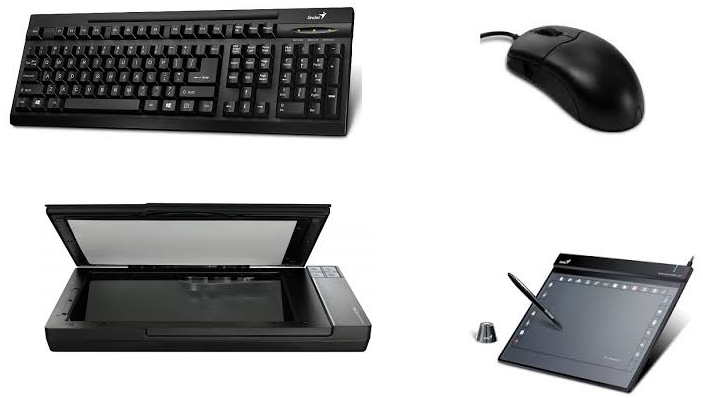
\includegraphics[width=0.9\textwidth, keepaspectratio]{../figs/cap04/entrada} 
					
				\end{figure}
			\end{column}
		\end{columns}
	
	\end{frame}
	
	\begin{frame}
		\frametitle{Periféricos de saída}
		\begin{columns}
			\begin{column}{0.35\textwidth}
				\vspace{-1cm}
				\begin{itemize}
					\item Impressora
					\item Monitor
					\item \textit{Plotter}
					
				\end{itemize}
			\end{column}
			\begin{column}{0.65\textwidth}
				\begin{figure}
					\centering
					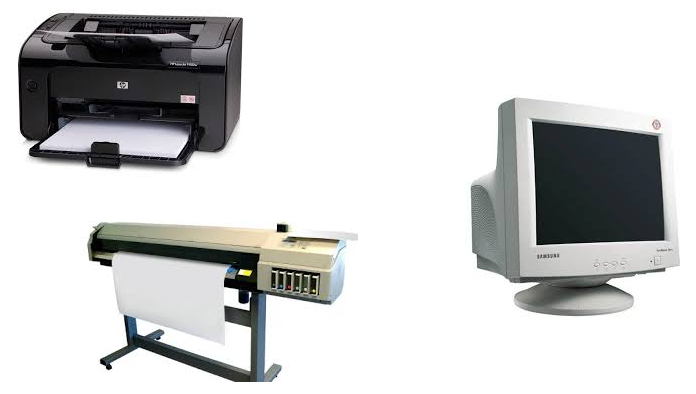
\includegraphics[width=0.9\textwidth, keepaspectratio]{../figs/cap04/saida} 
					
				\end{figure}
			\end{column}
		\end{columns}
	\end{frame}
	
	\section{Barramentos}
	
	\begin{frame}
		\frametitle{Barramentos}
		\begin{itemize}
			\item Vias que interligam os dispositivos (CPU, memória e periféricos), permitindo a comunicação entre os mesmos.
			\vspace{1em}
		\end{itemize}
		
		\begin{columns}[t]
			\begin{column}{0.35\textwidth}
				\begin{itemize}
				
					\item Três tipos
					\begin{itemize}
						\item Dados
						\item Endereços
						\item Controle				
					\end{itemize}
				\end{itemize}
			\end{column}
			\begin{column}{0.65\textwidth}
				\begin{figure}
					\centering
					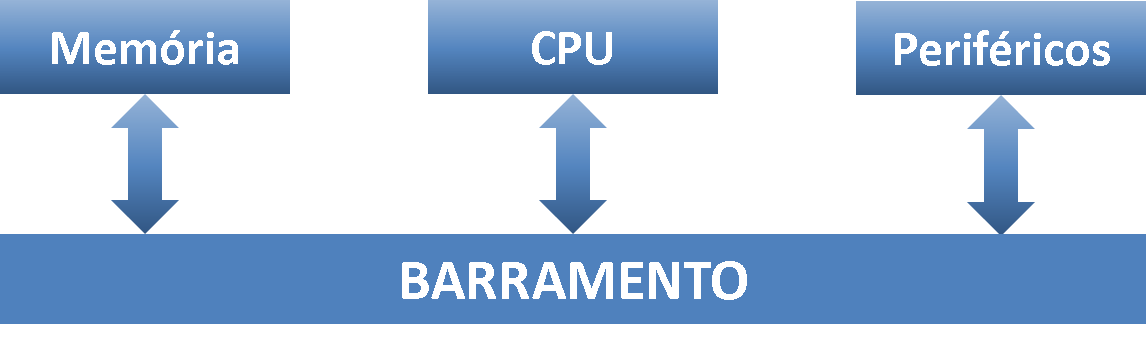
\includegraphics[width=.9\textwidth, keepaspectratio]{../figs/cap04/barramento} 					
				\end{figure}			
			\end{column}
		\end{columns}
		

	\end{frame}
	
	\section{Modelos de Arquitetura}
	
	\begin{frame}
		\frametitle{Modelos de Arquiteturas}
		\begin{itemize}
			\item Definem como os componentes do sistema estão interligados
			\vspace{1em}
			\item Dois modelos
			\begin{itemize}
				\item Von Neumann
				\item Harvard
			\end{itemize}
			\vspace{1em}
			\item Principais diferenças
			\begin{itemize}
				\item Organização de memória
				\item Uso dos barramentos
	
			\end{itemize}
		\end{itemize}
	\end{frame}
	
	\begin{frame}
		\frametitle{Arquitetura Von Neumann}
			\begin{itemize}
				\item Arquitetura mais comum nos microprocessadores utilizados em computadores pessoais
				\vspace{1em}
				\item Memória de dados e de programa compartilham o mesmo barramento de dados e de endereço

			\end{itemize}	

	\end{frame}

	\begin{frame}
		\frametitle{Arquitetura Von Neumann}
		\begin{figure}
		\centering
			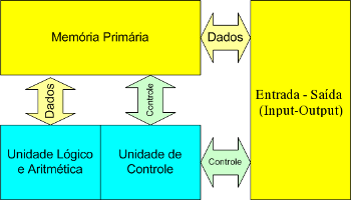
\includegraphics[height=0.7\textheight, keepaspectratio]{../figs/cap04/neumann} 
			
		\end{figure}
	\end{frame}

	\begin{frame}
		\frametitle{Arquitetura Harvard}
			\begin{itemize}
				\item Mais utilizada em microcontroladores

				\vspace{1em}
				\item Memória de dados e de programa são separadas, podendo possuir capacidades diferentes de armazenamento
				
				\vspace{1em}
				\item Barramentos exclusivos para cada tipo de memória (programa e dados)



			\end{itemize}	

	\end{frame}

	\begin{frame}
		\frametitle{Arquitetura Harvard}
				\begin{figure}
				\centering
					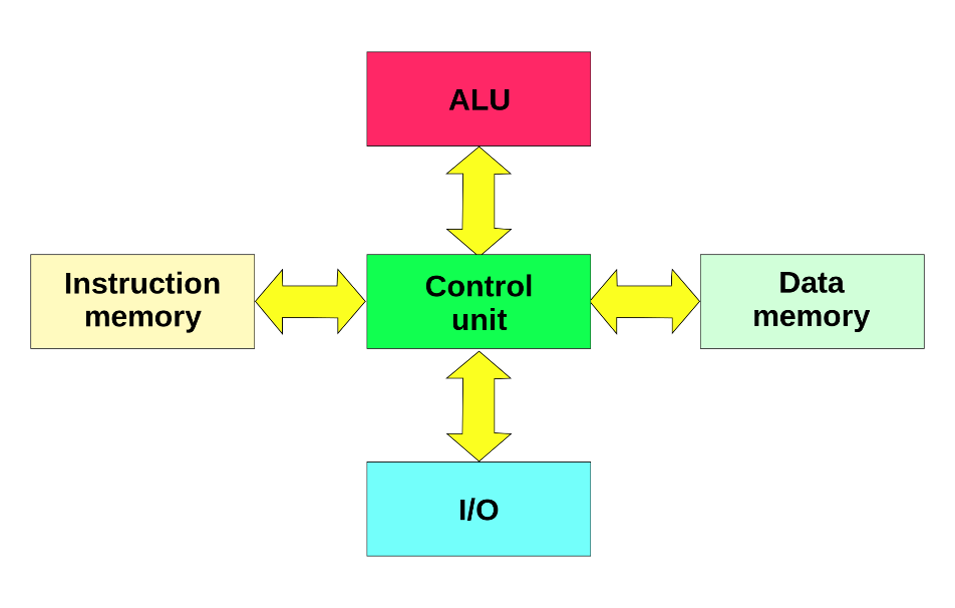
\includegraphics[height=0.85\textheight, keepaspectratio]{../figs/cap04/harvard} 
					
				\end{figure}
	\end{frame}
	
	\section{Exercícios}

	\begin{frame}
		\frametitle{Verdadeiro ou Falso}
		Considerando a organização e arquitetura de computadores, julgue os itens que se seguem. 
		
		\vspace{1em}
São funções básicas de um computador: processamento de dados, armazenamento de dados, transferência de dados e controle. São componentes estruturais de um computador: unidade central de processamento, memória principal, dispositivos de entrada e saída e sistemas de interconexão
	\end{frame}

	\begin{frame}
		Em relação à organização dos sistemas computacionais, as alternativas abaixo apresentam os principais componentes, EXCETO: 
		
		\vspace{1em}
		\begin{enumerate}[a]
			\normalsize
			\item Componentes de E/S.
			\item Sistema operacional.
			\item Memória.
			\item Processador.
		\end{enumerate}
	\end{frame}

	\begin{frame}
		Em relação aos componentes básicos dos microcomputadores, aquele que fornece a sincronização e a ordenação de operações, necessária para a execução correta de programas é: 
		
		\vspace{1em}
		\begin{enumerate}[a]
			\normalsize
			\item  Unidade Aritmética e Lógica.
			\item  Unidade Central de Processamento. 
			\item  Registradores.
			\item  Unidade de Controle.
			\item  Unidade de Armazenamento. 
		\end{enumerate}

	\end{frame}
	
	\begin{frame}
		\frametitle{Verdadeiro ou Falso}
		Julgue o item subsequente acerca dos componentes de um computador, dos sistemas de entrada, saída e armazenamento e dos princípios de sistemas operacionais. 
		
		\vspace{1em}
		Um dos componentes do computador é a unidade lógica e aritmética (ULA), parte integrante da unidade de controle (UC), que realiza, em regra, operações matemáticas complexas.

	\end{frame}
	
	\begin{frame}
		Na configuração de microcomputadores versão desktop, são inseridos diversos dispositivos de entrada e saída de dados, cada um com uma função específica. Nesse sentido, dependendo do momento em que são utilizados, podem realizar a função de entrada em um instante e de saída de dados, em outro. São exemplos de dispositivos que se enquadram nessa categoria: 
		
		\vspace{1em}
		\begin{enumerate}[a]
			\normalsize
			\item mouse e impressora deskjet.
			\item blu-ray e impressora térmica.
			\item teclado e impressora laserjet.
			\item pendrive e impressora multifuncional.
		\end{enumerate}
	\end{frame}	
	
	\begin{frame}
		Observe a afirmação a seguir e, em seguida, escolha a alternativa que completa corretamente as lacunas:
		
		\vspace{1em}
		Na Arquitetura de von Neumann, uma Unidade de Processamento Central (CPU) é composta por uma ___________ e uma ___________.
		
		\vspace{1em}
		\begin{enumerate}[a]
			\normalsize
			\item memória RAM; tabela de endereçamento.
			\item unidade de entrada; unidade de saída.
			\item unidade de memória; unidade de entrada.
			\item unidade de controle; unidade aritmética e lógica (ULA).
			\item tabela de endereçamento; unidade de controle.

		\end{enumerate}
	\end{frame} 
	
	\begin{frame}
		Segundo o conceito da Máquina de Von Neumann
		
		\vspace{1em}
		\begin{enumerate}[a]
			\normalsize
			\item apenas instruções ficam armazenadas.
			\item instruções e dados são armazenados na mesma memória.
			\item instruções e dados são armazenados em memórias distintas.
			\item instruções e dados não são armazenados, com vistas à otimização do uso da memória.
			\item os dados ficam armazenados na memória, não havendo armazenamento de instruções.
		\end{enumerate}
	\end{frame}
	
	\begin{frame}
		Com relação aos elementos de um computador e à sua arquitetura básica, assinale a opção correta.

		\vspace{1em}
		\begin{enumerate}[a]
			\normalsize
			\item O processador - ou microprocessador - é responsável pelas entradas e pelas saídas de dados do computador.
			\item A unidade central de processamento é responsável pela armazenagem dos programas e dos dados.
			\item Os periféricos são os dispositivos responsáveis pelo tratamento de informações armazenadas em memória, tanto de programas em código de máquina quanto dos dados.
			\item Barramento é uma via de comunicação de alto desempenho por onde circulam os dados tratados pelo computador.
		\end{enumerate}

	\end{frame}
	
	\begin{frame}{Bibliografia}
		\nocite{Englander2011}
		\nocite{Paixao2014}
		\nocite{Stallings2010}
    	\bibliographystyle{plain}
    	\bibliography{../refs}   	
	
	\end{frame}
		
	\begin{frame}{}
	\end{frame}
\end{document}